\chapter{Θεωρητικό υπόβαθρο}
\InitialCharacter{Σ}το κεφάλαιο αυτό παρουσιάζονται η εξέλιξη του 
\en{Cloud Computing}, η τεχνολογία \en{Blockchain}, καθώς και οι
αποκεντρωμένες εφαρμογές. Επίσης, γίνεται αναφορά σε προηγούμενες εργασίες 
που ασχολούνται με την ιδέα του αποκεντρωμένου υπολογιστικού νέφους.

\section{\en{Cloud Computing}}
\subsection{Εξέλιξη \en{Cloud Computing}}
Το υπολογιστικό νέφος αφορά την παροχή διαφόρων υπηρεσιών μέσω του 
διαδικτύου, συμπεριλαμβανομένων της αποθήκευσης και της υπολογιστικής ισχύος. 
Η έννοια, αν και έγινε ευρέως διαδεδομένη τα τελευταία χρόνια, έχει τις ρίζες 
της στην δεκαετία του 1960 με την έλευση του \en{utility computing}. Η ιδέα 
βασιζόταν στο εγχείρημα ότι οι υπολογιστικοί πόροι, όπως το νερό και το 
ηλεκτρικό ρεύμα, μπορούν να παρέχονται σε οικίες και επιχειρήσεις ως υπηρεσία 
κοινής ωφέλειας. Ωστόσο, μόλις την δεκαετία του 2000, με την άνοδο του 
διαδικτύου υψηλής ταχύτητας, τις σημαντικές εξελίξεις στις τεχνολογίες
της εικονικοποί-ησης \en{(virtualization)} και την αύξηση της υπολογιστικής ισχύος, 
το \en{cloud computing} άρχισε να παίρνει την σύγχρονη μορφή του. 

Εταιρείες όπως η \en{Amazon}, η \en{Microsoft}, η \en{IBM} και η \en{Google}, ήταν από τις 
πρώτες που αναγνώρισαν τις δυνατότητες ενοικίασης των τεράστιων υπολογιστικών 
πόρων τους \cite{ref1} . Η \en{Amazon Web Services (AWS)} ξεκίνησε το 2006, σηματοδοτώντας 
την έναρξη της σύγχρονης εποχής του νέφους. Τα επόμενα χρόνια παρατηρήθηκε 
μια έκρηξη υπηρεσιών \en{cloud computing} \cite{ref2}, οι οποίες καλύπτουν διάφορες τεχνολογικές ανάγκες, 
από την υποδομή ως υπηρεσία \en{(Infrastructure as a Service – IaaS)} έως το 
λογισμικό ως υπηρεσία \en{(Software as a Service – SaaS)}.

\subsection{Υφιστάμενα συγκεντρωτικά μοντέλα και οι περιορισμού τους}
Τα συγκεντρωτικά μοντέλα υπολογιστικού νέφους, προσφερόμενα από τεχνολογικούς 
κολοσσούς όπως το \en{AWS}, το \en{Google Cloud} και το \en{Microsoft Azure}
κυριαρχούν στην τρέχουσα αγορά. Οι υπηρεσίες αυτές παρέχουν στους χρήστες 
αξιόπιστες, κλιμακούμενες και συχνά οικονομικά αποδοτικές λύσεις. 

Ωστόσο, συνοδεύονται από εγγενείς περιορισμούς:
\begin{itemize}
\item Έλλειψη διαφάνειας: Ο τρόπος τιμολόγησης μπορεί να είναι πολύπλοκος και οι 
χρήστες συχνά δεν έχουν σαφή εικόνα για την κατανομή των πόρων \cite{ref3,ref4,ref5} .
\item Ενιαίο σημείο αποτυχίας (\en{single point of failure}): Τα συγκεντρωτικά 
συστήματα, εκ κατασκευής, έχουν πιθανά σημεία συμφόρησης. Εάν ένας μεγάλος 
πάροχος υπηρεσιών υπολογιστικού νέφους αντιμετωπίσει διακοπή λειτουργίας, 
αυτό μπορεί να επηρεάσει μεγάλο πλήθος χρηστών.
\item Ανησυχίες σχετικά με το απόρρητο των δεδομένων: Με τα δεδομένα 
συγκεντρωμένα σε λίγες εταιρείες, υπάρχουν βάσιμες ανησυχίες σχετικά με την 
κατάχρηση των δεδομένων, την παρακολούθηση των χρηστών, καθώς και τις παραβιάσεις των υπαρχόντων συστημάτων.
\item Δυνατότητα μονοπωλιακής συμπεριφοράς: Η κυριαρχία λίγων εταιρειών στην 
αγορά μπορεί να οδηγήσει σε μείωση του ανταγωνισμού και της καινοτομίας.
\end{itemize}

Παράλληλα με τους παραπάνω περιορισμούς, τα \en{data centers} που χρησιμοποιούνται
για την παροχή των υπηρεσιών \en{cloud computing} καταναλώνουν μεγάλες ποσότητες
ενέργειας, με αρνητικές επιπτώσεις στο περιβάλλον \cite{ref40, ref41}. 

\subsection{\en{Serverless Computing}}
Με τον όρο \en{serveless computing} αναφερόμαστε σε ένα μοντέλο υπολογιστικού νέφους, στο οποίο οι προγραμματιστές δεν χρειάζεται να διαχειρίζονται οι ίδιοι τους πόρους και την υποδομή του \en{server} τους, επιτρέποντάς τους να επικεντρώνονται στον κώδικα του προγράμματός τους \cite{ref6}. Αντί να υπάρχει μονίμως ενεργός ένας \en{server}, αυτός εκκινείται όταν ληφθεί ένα συγκεκριμένο \en{event}, εκτελεί την επιθυμητή συνάρτηση και, μόλις αυτή ολοκληρωθεί, τερματίζει την λειτουργία του. Το μοντέλο αυτό χαρακτηρίζεται από αυτόματη κλιμάκωση και μειωμένο κόστος εκτέλεσης, καθώς οι χρήστες χρεώνονται μόνο για την πραγματική τους χρήση, συνήθως με βάση τον αριθμό και τον χρόνο εκτέλεσης της συνάρτησής τους. Έτσι, η διαδικασία ανάπτυξης εφαρμογών επιταχύνεται, μειώνοντας ταυτόχρονα το κόστος και την λειτουργική πολυπλοκότητα \cite{ref7,ref8}. 


\section{\en{Blockchain}}
\subsection{Εισαγωγή στην τεχνολογία \en{Blockchain}}
Το 2008, μια οντότητα - άνθρωπος ή ομάδα ανθρώπων - με το ψευδώνυμο \en{Satoshi Nakamoto} παρουσίασε το \en{Bitcoin}, ένα αποκεντρωμένο ψηφιακό νόμισμα \cite{ref9}. Πέρα από τη νομισματική του λειτουργία, το \en{Bitcoin} εισήγαγε την τεχνολογία του \en{Blockchain}. 
Το \en{Blockchain} είναι μια αλυσίδα από \en{blocks}, στα οποία αποθηκεύονται οι συναλλαγές που πραγματοποιούνται στο δίκτυο. Αποτελεί, δηλαδή, μια βάση δεδομένων συναλλαγών σε ένα δίκτυο, η οποία λειτουργεί ως αποκεντρωμένο λογιστικό βιβλίο. Προσφέρει διαφάνεια, ασφάλεια και απουσία κεντρικού ελέγχου. Στον πυρήνα του, το \en{Blockchain}, χρησιμοποιώντας κρυπτογραφικές αποδείξεις και έναν αλγόριθμο συναίνεσης (\en{consensus algorithm}) \cite{ref10} \\είναι ανθεκτικό στην τροποποίηση των δεδομένων του, διατηρώντας με τον τρόπο αυτό την ακεραιότητά τους, και εξασφαλίζοντας την εμπιστοσύνη μεταξύ των συμμετεχόντων. 

\begin{illustration}
    \centering
    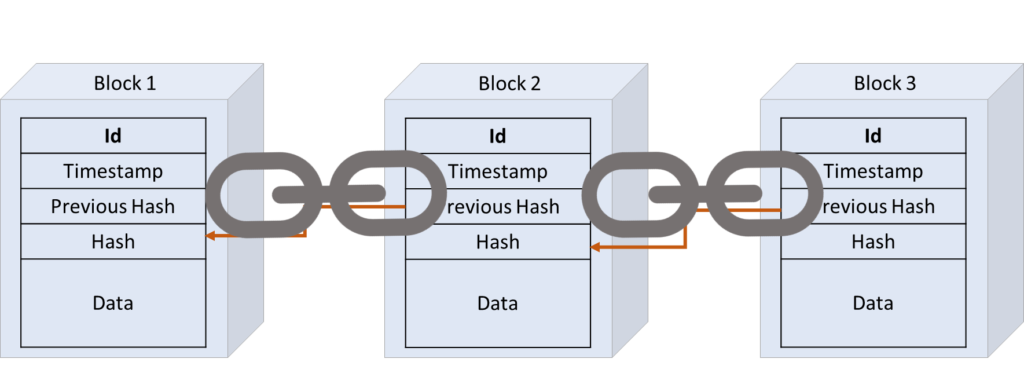
\includegraphics[width=0.7\textwidth]{figures/figure-001.png}
    \caption{Γραφική απεικόνιση του \en{Blockchain}} 
    \cite{ref11} 
\end{illustration}


\subsection{\en{Ethereum}}
To \en{Ethereum}, το οποίο παρουσιάστηκε το 2013 από τον \en{Vitalik Buterin} και δημοσιεύθηκε το 2015, επέκτεινε την ιδέα του \en{Blockchain} και δημιούργησε μια δημόσια,ανοικτού κώδικα, πλατφόρμα κατανεμημένου υπολογισμού, η οποία διαθέτει την λειτουργικότητα των έξυπνων συμβολαίων \cite{ref12,ref13}. Με τον τρόπο αυτό, παρέχει στους προγραμματιστές την \en{Ethereum Virtual Machine (EVM)}, μια αποκεντρωμένη εικονική μηχανή που είναι \en{Turing complete}, μετατρέποντας τη δημιουργία εφαρμογών στο \en{Blockchain} σε πολύ απλούστερη και εύκολη διαδικασία \cite{ref14}.


\subsection{Έξυπνα συμβόλαια και Aποκεντρωμένες εφαρμογές}
Μία από τις βασικές καινοτομίες του \en{Ethereum} είναι το έξυπνο συμβόλαιο (\en{smart contract}). Τα έξυπνα συμβόλαια είναι ντετερμινιστικά αυτοεκτελούμενα συμβόλαια όπου οι όροι γράφονται απευθείας σε κώδικα και διανέμονται στο \en{Blockchain} \cite{ref14,ref15}. Εκτελούν αυτόματα αξιόπιστες συναλλαγές, χωρίς την ανάγκη διαμεσολάβησης τρίτου, με τρόπο ανιχνεύσιμο και μη αναστρέψιμο. Η προσθήκη των έξυπνων συμβολαίων επεκτείνει την χρήσης της τεχνολογίας \en{Blockchain} πέρα από τις χρηματοοικονομικές συναλλαγές - όπως αυτές στις οποίες απευθύνεται το \en{Bitcoin} - σε οποιονδήποτε τομέα η εμπιστοσύνη είναι απαραίτητη, όπως τα συστήματα ψηφοφορίας και οι εφαρμογές \en{Internet of Things (IoT)} \cite{ref16}.

Οι αποκεντρωμένες εφαρμογές, ή \en{dApps} \cite{ref17,ref18}, είναι ένα άμεσο προϊόν της λειτουργικότητας των έξυπνων συμβολαίων, που εκτελούνται σε ένα δίκτυο \en{Blockchain} με ομότιμο τρόπο. Αυτές οι εφαρμογές δεν απαιτούν κεντρική αρχή, είναι ανοικτού κώδικα και δίνουν κίνητρα στους χρήστες μέσω κρυπτογραφικών \en{tokens}. Αξιοποιούν τα οφέλη της τεχνολογίας \en{Blockchain} για να διασφαλίσουν ότι καμία μεμονωμένη οντότητα δεν έχει τον έλεγχο της εφαρμογής, προσφέροντας ένα νέο επίπεδο ασφάλειας και εμπιστοσύνης για τους χρήστες.


\subsection{\en{Web 3.0}}
Με βάση τα \en{dApps}, το \en{Web3} προτάθηκε το 2014 από τον συνιδρυτή του \en{Ethereum}, \en{Gavin Wood}, ως ένα νέο μοντέλο χρήσης του διαδικτύου. Αναγνωρίζοντας ότι το παρόν μοντέλο του διαδικτύου (\en{Web 2.0}) προϋποθέτει την εμπιστοσύνη των χρηστών προς κεντρικούς παρόχους, προτείνεται η χρήση του \en{Blockchain} για την κατασκευή μιας νέας, αποκεντρωμένης έκδοσής του, στην οποία τον έλεγχο των δεδομένων κατέχουν οι ίδιοι οι χρήστες \cite{ref19}.

\begin{illustration}
    \centering
    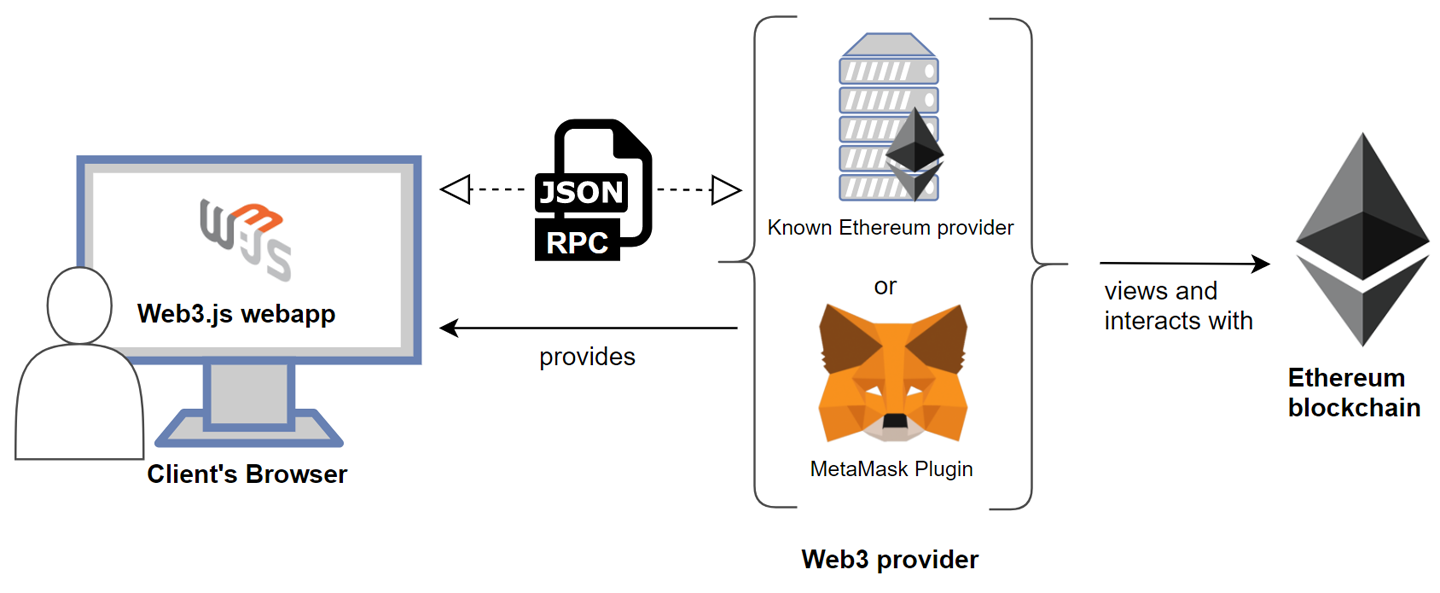
\includegraphics[width=0.7\textwidth]{figures/figure-002.png}
    \caption{Αρχιτεκτονική του \en{Web3}} 
    \cite{ref14} 
\end{illustration}

\subsection{\en{Ether} και \en{Gas Fees}}
Το \en{token} του \en{Ethereum}, το \en{Ether} (\en{ETH}), εξυπηρετεί δύο βασικούς σκοπούς: την αποζημίωση των κόμβων του δικτύου για τους υπολογισμούς που εκτελούν και τη διαπραγμάτευσή του ως ψηφιακό νόμισμα σε διάφορα ανταλλακτήρια κρυπτονομισμάτων \cite{ref20}. Στο δίκτυο του \en{Ethereum}, οι αμοιβές των συναλλαγών μετρώνται με βάση την υπολογιστική πολυπλοκότητα, τη χρήση εύρους ζώνης και τις ανάγκες αποθήκευσης, οι οποίες υπολογίζονται σε όρους \en{gas} και πληρώνονται σε \en{ETH}. Αυτό διασφαλίζει ότι κακόβουλα προγράμματα ή αναποτελεσματικός κώδικας δεν φράσσουν το δίκτυο \cite{ref21}.

Για να διευκολύνει τις συναλλαγές και τους υπολογισμούς, το \en{Ethereum} χρησιμοποιεί και μονάδες μικρότερης αξίας. Η μικρότερη μονάδα του \en{Ether} είναι γνωστή ως \en{wei}. Ένα \en{Ether} ισοδυναμεί με ένα πεντάκις εκατομμύριο \en{wei} ($1 \en{wei} = 10^{-18} \en{eth}$). H αμέσως επόμενη μονάδα που χρησιμοποιείται ονομάζεται \en{gwei} (\en{Gigawei}) και ισοδυναμεί με ένα δισεκατομμύριο \en{wei} ή 0,000000001 \en{Ether}.

Αυτές οι μικρότερες μονάδες \en{Ether} είναι σημαντικές για την ακρίβεια στις συναλλαγές, ειδικά όταν πρόκειται για χρεώσεις \en{gas}, καθώς επιτρέπουν στους χρήστες να καθορίζουν το ακριβές ποσό που είναι διατεθειμένοι να πληρώσουν ανά μονάδα \en{gas}, χωρίς να χρειάζεται να χρησιμοποιούν εξαιρετικά μικρής αξίας δεκαδικά ψηφία. Αυτό το σύστημα όχι μόνο παρέχει μια πιο κατανοητή κλίμακα για τους χρήστες, αλλά επιτρέπει επίσης στο δίκτυο \en{Ethereum} να χειρίζεται τις συναλλαγές και τις αλληλεπιδράσεις έξυπνων συμβολαίων με ακρίβεια, εξασφαλίζοντας δικαιοσύνη για όλα τα εμπλεκόμενα μέρη.

\subsection{\en{Ethereum} 2.0}
Αρχικά, το \en{Ethereum Blockchain} χρησιμοποιούσε ως αλγόριθμο συναίνεσης (\en{consensus algorithm}) το \en{Proof of Work (PoW)} που χρησιμοποιεί και το \en{Bitcoin}. Το γεγονός αυτό εισήγαγε περιορισμούς στην επεκτασιμότητα του δικτύου, την ενεργειακή αποδοτικότητά του, καθώς και υψηλές χρεώσεις στις συναλλαγές. Στις 15 Σεπτεμβρίου 2022, ολοκληρώθηκε η μετάβαση στο \en{Blockchain Ethereum} 2.0, το οποίο χρησιμοποιεί για \en{consensus algorithm} το \en{Proof of Stake (PoS)}, μειώνοντας έτσι την ενεργειακή κατανάλωση κατά 99\% \cite{ref22}. 

\subsection{\en{Layer 2}}
Οι τρεις επιθυμητές ιδιότητες της τεχνολογίας \en{Blockchain} είναι η αποκέντρωση, η ασφάλεια και η επεκτασιμότητα. Ωστόσο, σύμφωνα με το \en{Blockchain Trilemma} \cite{ref23}, μια απλή αρχιτεκτονική του μπορεί να πετύχει μόνο δύο από τις τρεις. Έτσι, προς επίτευξη ενός ασφαλούς και αποκεντρωμένου δικτύου, πρέπει να θυσιαστεί η επεκτασιμότητα. 

Καθώς το \en{Ethereum} επεξεργάζεται σήμερα περισσότερες από 1 εκατομμύριο συναλλαγές την ημέρα, με δυνατότητα επεξεργασίας 15 συναλλαγές το δευτερόλεπτο, η συνεχώς αυξανόμενη ζήτηση για χρήση του μπορεί να προκαλέσει υψηλές χρεώσεις στις συναλλαγές.
Στο σημείο αυτό εισάγονται τα δίκτυα επιπέδου 2 (\en{layer} 2), τα οποία, ενώ χρησιμοποιούν το δίκτυο του επιπέδου 1 (\en{mainnet Ethereum}), παρέχουν τρόπους για επεξεργασία των συναλλαγών εκτός αυτού (\en{off-chain computations}). Έτσι, αφαιρούν το βάρος επιβεβαίωσης κάθε συναλλαγής από το επίπεδο 1, επιτρέποντάς του να γίνει λιγότερο συμφορημένο και όλα να γίνονται πιο κλιμακούμενα, χωρίς να θυσιάζεται η αποκέντρωση και η ασφάλεια \cite{ref24}. 



\section{Προηγούμενες εργασίες σχετικά με το αποκεντρωμένο \en{cloud computing} και τις \en{dApps}}
Οι περιορισμοί των συγκεντρωτικών μοντέλων υπολογιστικού νέφους και οι 
δυνατότητες της τεχνολογίας \en{Blockchain}, οδήγησαν ερευνητές και 
προγραμματιστές να εξερευνήσουν το αποκεντρωμένο υπολογιστικό νέφος \cite{ref25,ref26,ref27,ref28,ref29,ref30}. Έργα τα οποία έχουν αποτολμήσει το εγχείρημα αυτό, με στόχο την δημιουργία μιας 
αποκεντρωμένης αγοράς υπολογιστικής ισχύος και κατανεμημένου αποθηκευτικού 
χώρου είναι:

\begin{itemize}
    \item Το \en{SONM}: Μια αποκεντρωμένη πλατφόρμα που προσφέρει σε χρήστες την ευκαιρία να νοικιάσουν τους αδρανείς υπολογιστικούς πόρους τους, δημιουργώντας ένα δίκτυο ομότιμων κόμβων. Ο κεντρικός στόχος της πλατφόρμας είναι η παροχή υποδομής (\en{IaaS}) κυρίως για εφαρμογές μηχανικής μάθησης και \en{video rendering}, τα οποία απαιτούν μεγάλη υπολογιστική ισχύ \cite{ref31}.
    \item To \en{Golem}: Μια πλατφόρμα που έχει σκοπό την δημιουργία ενός αποκεντρωμένου υπερυπολογιστή. Απευθύνεται κυρίως σε χρήστες με απαιτητικές εργασίες, όπως η βαθιά μάθηση και η επεξεργασία γραφικών \cite{ref32}.
    \item Το \en{iExec}: Μια αποκεντρωμένη πλατφόρμα βασισμένη στο \en{Ethereum}, η οποία χρησιμοποιεί του αδρανείς πόρους του υπολογιστή για την επεξεργασία δεδομένων. Για την επιλογή των παρόχων που θα εκτελέσουν την εργασία χρησιμοποιείται \en{task scheduler} \cite{ref33}.
    \item Το \en{Filecoin}: Μια αποκεντρωμένη πλατφόρμα και πρωτόκολλο για την αποθήκευση δεδομένων, η οποία προσφέρει την \en{Filecoin Virtual Machine} για την ανάπτυξη εφαρμογών στο δίκτυό της \cite{ref34}.
    \item Το \en{CloudAgora}: Μια πλατφόρμα που στοχεύει να σπάσει 
    το μονοπώλιο των παραδοσιακών παρόχων υπολογιστικού νέφους. Αξιοποιεί 
    την τεχνολογία \en{Blockchain} για να προσφέρει μια αποκεντρωμένη αγορά 
    υπολογιστικών πόρων και αποθήκευσης, επιτρέποντας σε οποιονδήποτε δυνητικό 
    πάροχο πόρων να χρησιμοποιεί τους αδρανείς πόρους του και να ανταγωνίζεται με 
    τους υπόλοιπους με ίσους όρους. Στην περίπτωση της εκτέλεσης εργασίας με 
    υπολογιστικούς πόρους, για την επαλήθευση της ορθής εκτέλεσής της, 
    χρησιμοποιεί το \en{TrueBit Protocol} \cite{ref35} το οποίο αποτελεί μια σύνθετη επιλογή που προσθέτει καθυστέρηση στην εκτέλεση των εργασιών και αυξάνει το κόστος των συναλλαγών. Για την εκτέλεση των εργασιών, επιλέγεται πάντοτε ο πάροχος που θα έχει υποβάλει την καλύτερη προσφορά \cite{ref36,ref37}.
    \item Το \en{ChainFaas}: Μια πλατφόρμα που στοχεύει στην αξιοποίηση της υπολογιστικής ικανότητας 
    των προσωπικών υπολογιστών για εργασίες υπολογιστικής ισχύος. Δεν ελέγχει την ορθή εκτέλεση της εργασίας από τον πάροχο, αλλά χρησιμοποιεί ιδιωτικό (\en{private}) \en{Blockchain} για την σύνδεση παρόχων και πελατών. Η επιλογή του παρόχου γίνεται με \en{task scheduler} \cite{ref38,ref39}.
\end{itemize}
